\documentclass[twoside]{book}

% Packages required by doxygen
\usepackage{fixltx2e}
\usepackage{calc}
\usepackage{doxygen}
\usepackage[export]{adjustbox} % also loads graphicx
\usepackage{graphicx}
\usepackage[utf8]{inputenc}
\usepackage{makeidx}
\usepackage{multicol}
\usepackage{multirow}
\PassOptionsToPackage{warn}{textcomp}
\usepackage{textcomp}
\usepackage[nointegrals]{wasysym}
\usepackage[table]{xcolor}

% Font selection
\usepackage[T1]{fontenc}
\usepackage[scaled=.90]{helvet}
\usepackage{courier}
\usepackage{amssymb}
\usepackage{sectsty}
\renewcommand{\familydefault}{\sfdefault}
\allsectionsfont{%
  \fontseries{bc}\selectfont%
  \color{darkgray}%
}
\renewcommand{\DoxyLabelFont}{%
  \fontseries{bc}\selectfont%
  \color{darkgray}%
}
\newcommand{\+}{\discretionary{\mbox{\scriptsize$\hookleftarrow$}}{}{}}

% Page & text layout
\usepackage{geometry}
\geometry{%
  a4paper,%
  top=2.5cm,%
  bottom=2.5cm,%
  left=2.5cm,%
  right=2.5cm%
}
\tolerance=750
\hfuzz=15pt
\hbadness=750
\setlength{\emergencystretch}{15pt}
\setlength{\parindent}{0cm}
\setlength{\parskip}{3ex plus 2ex minus 2ex}
\makeatletter
\renewcommand{\paragraph}{%
  \@startsection{paragraph}{4}{0ex}{-1.0ex}{1.0ex}{%
    \normalfont\normalsize\bfseries\SS@parafont%
  }%
}
\renewcommand{\subparagraph}{%
  \@startsection{subparagraph}{5}{0ex}{-1.0ex}{1.0ex}{%
    \normalfont\normalsize\bfseries\SS@subparafont%
  }%
}
\makeatother

% Headers & footers
\usepackage{fancyhdr}
\pagestyle{fancyplain}
\fancyhead[LE]{\fancyplain{}{\bfseries\thepage}}
\fancyhead[CE]{\fancyplain{}{}}
\fancyhead[RE]{\fancyplain{}{\bfseries\leftmark}}
\fancyhead[LO]{\fancyplain{}{\bfseries\rightmark}}
\fancyhead[CO]{\fancyplain{}{}}
\fancyhead[RO]{\fancyplain{}{\bfseries\thepage}}
\fancyfoot[LE]{\fancyplain{}{}}
\fancyfoot[CE]{\fancyplain{}{}}
\fancyfoot[RE]{\fancyplain{}{\bfseries\scriptsize Generated by Doxygen }}
\fancyfoot[LO]{\fancyplain{}{\bfseries\scriptsize Generated by Doxygen }}
\fancyfoot[CO]{\fancyplain{}{}}
\fancyfoot[RO]{\fancyplain{}{}}
\renewcommand{\footrulewidth}{0.4pt}
\renewcommand{\chaptermark}[1]{%
  \markboth{#1}{}%
}
\renewcommand{\sectionmark}[1]{%
  \markright{\thesection\ #1}%
}

% Indices & bibliography
\usepackage{natbib}
\usepackage[titles]{tocloft}
\setcounter{tocdepth}{3}
\setcounter{secnumdepth}{5}
\makeindex

% Hyperlinks (required, but should be loaded last)
\usepackage{ifpdf}
\ifpdf
  \usepackage[pdftex,pagebackref=true]{hyperref}
\else
  \usepackage[ps2pdf,pagebackref=true]{hyperref}
\fi
\hypersetup{%
  colorlinks=true,%
  linkcolor=blue,%
  citecolor=blue,%
  unicode%
}

% Custom commands
\newcommand{\clearemptydoublepage}{%
  \newpage{\pagestyle{empty}\cleardoublepage}%
}

\usepackage{caption}
\captionsetup{labelsep=space,justification=centering,font={bf},singlelinecheck=off,skip=4pt,position=top}

%===== C O N T E N T S =====

\begin{document}

% Titlepage & ToC
\hypersetup{pageanchor=false,
             bookmarksnumbered=true,
             pdfencoding=unicode
            }
\pagenumbering{alph}
\begin{titlepage}
\vspace*{7cm}
\begin{center}%
{\Large Configurable\+Menus }\\
\vspace*{1cm}
{\large Generated by Doxygen 1.8.13}\\
\end{center}
\end{titlepage}
\clearemptydoublepage
\pagenumbering{roman}
\tableofcontents
\clearemptydoublepage
\pagenumbering{arabic}
\hypersetup{pageanchor=true}

%--- Begin generated contents ---
\chapter{Hierarchical Index}
\section{Class Hierarchy}
This inheritance list is sorted roughly, but not completely, alphabetically\+:\begin{DoxyCompactList}
\item Command\+Executor\begin{DoxyCompactList}
\item \contentsline{section}{A\+P\+I.\+Menu\+Manager}{\pageref{class_a_p_i_1_1_menu_manager}}{}
\end{DoxyCompactList}
\item Listener\begin{DoxyCompactList}
\item \contentsline{section}{A\+P\+I.\+Configurable\+Menu}{\pageref{class_a_p_i_1_1_configurable_menu}}{}
\end{DoxyCompactList}
\end{DoxyCompactList}

\chapter{Class Index}
\section{Class List}
Here are the classes, structs, unions and interfaces with brief descriptions\+:\begin{DoxyCompactList}
\item\contentsline{section}{\hyperlink{class_a_p_i_1_1_configurable_menu}{A\+P\+I.\+Configurable\+Menu} }{\pageref{class_a_p_i_1_1_configurable_menu}}{}
\item\contentsline{section}{\hyperlink{class_a_p_i_1_1_menu_manager}{A\+P\+I.\+Menu\+Manager} }{\pageref{class_a_p_i_1_1_menu_manager}}{}
\end{DoxyCompactList}

\chapter{Class Documentation}
\hypertarget{class_a_p_i_1_1_configurable_menu}{}\section{A\+P\+I.\+Configurable\+Menu Class Reference}
\label{class_a_p_i_1_1_configurable_menu}\index{A\+P\+I.\+Configurable\+Menu@{A\+P\+I.\+Configurable\+Menu}}
Inheritance diagram for A\+P\+I.\+Configurable\+Menu\+:\begin{figure}[H]
\begin{center}
\leavevmode
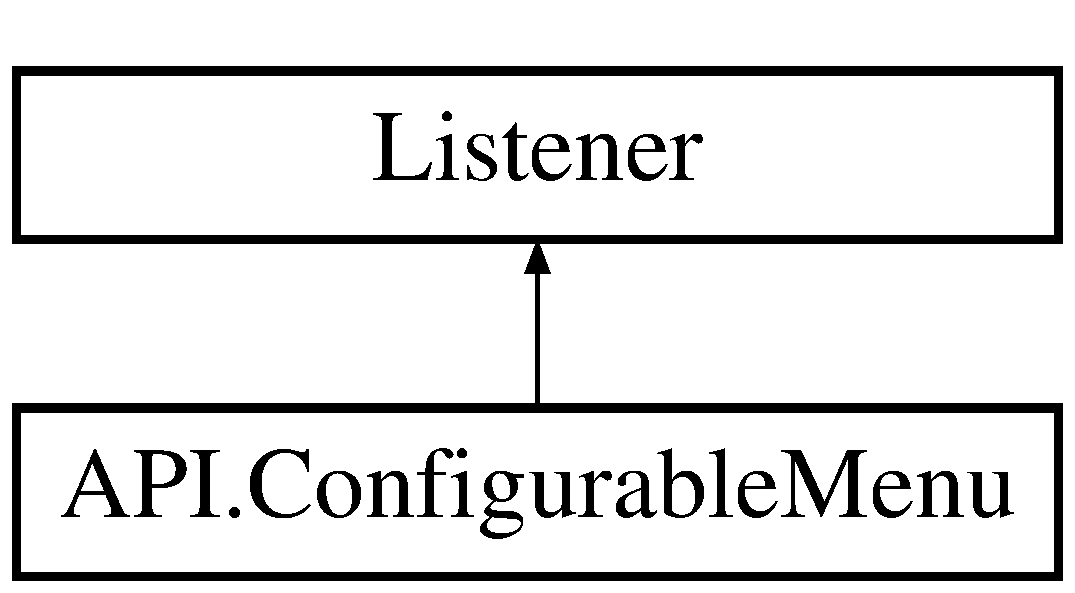
\includegraphics[height=2.000000cm]{class_a_p_i_1_1_configurable_menu}
\end{center}
\end{figure}
\subsection*{Public Member Functions}
\begin{DoxyCompactItemize}
\item 
\mbox{\Hypertarget{class_a_p_i_1_1_configurable_menu_ad93a4169815f31670e1fa7f2b7394f06}\label{class_a_p_i_1_1_configurable_menu_ad93a4169815f31670e1fa7f2b7394f06}} 
{\bfseries Configurable\+Menu} (String title, int rows)
\item 
\mbox{\Hypertarget{class_a_p_i_1_1_configurable_menu_ad3245c6614752c20cbff49cad0b5ebc5}\label{class_a_p_i_1_1_configurable_menu_ad3245c6614752c20cbff49cad0b5ebc5}} 
String {\bfseries get\+Name} ()
\item 
\mbox{\Hypertarget{class_a_p_i_1_1_configurable_menu_a274f2bcf031a3cd151395b5086dfffd0}\label{class_a_p_i_1_1_configurable_menu_a274f2bcf031a3cd151395b5086dfffd0}} 
String {\bfseries get\+Title} ()
\item 
\mbox{\Hypertarget{class_a_p_i_1_1_configurable_menu_acfb59e184a2cf28e6813272d72673da5}\label{class_a_p_i_1_1_configurable_menu_acfb59e184a2cf28e6813272d72673da5}} 
int {\bfseries get\+Rows} ()
\item 
\mbox{\Hypertarget{class_a_p_i_1_1_configurable_menu_a47cf45c112156a2c731bce39e1abe706}\label{class_a_p_i_1_1_configurable_menu_a47cf45c112156a2c731bce39e1abe706}} 
Item\+Stack {\bfseries get\+Slot} (int index)
\item 
\mbox{\Hypertarget{class_a_p_i_1_1_configurable_menu_a9f60e47822b4231d688114c627332d0c}\label{class_a_p_i_1_1_configurable_menu_a9f60e47822b4231d688114c627332d0c}} 
void {\bfseries delete\+Slot} (int index)
\item 
\mbox{\Hypertarget{class_a_p_i_1_1_configurable_menu_a61167dfe546ae011949531b34f551bee}\label{class_a_p_i_1_1_configurable_menu_a61167dfe546ae011949531b34f551bee}} 
void {\bfseries fill} (int from, int till, Item\+Stack item)
\item 
\mbox{\Hypertarget{class_a_p_i_1_1_configurable_menu_a33465b44c775dab604f35906d4df9f1a}\label{class_a_p_i_1_1_configurable_menu_a33465b44c775dab604f35906d4df9f1a}} 
void {\bfseries set\+Slot} (int index, Item\+Stack item)
\item 
\mbox{\Hypertarget{class_a_p_i_1_1_configurable_menu_a92f5b1dfe5d6ef2d958ae2d7dd8a874e}\label{class_a_p_i_1_1_configurable_menu_a92f5b1dfe5d6ef2d958ae2d7dd8a874e}} 
void {\bfseries fill} (int from, int till, Item\+Stack item, boolean clickable)
\item 
\mbox{\Hypertarget{class_a_p_i_1_1_configurable_menu_a5a654726058acf267a272ca5ed9ee052}\label{class_a_p_i_1_1_configurable_menu_a5a654726058acf267a272ca5ed9ee052}} 
void {\bfseries set\+Slot} (int index, Item\+Stack item, boolean clickable)
\item 
\mbox{\Hypertarget{class_a_p_i_1_1_configurable_menu_a6427862ff2f8ff423f4df4d4f5944804}\label{class_a_p_i_1_1_configurable_menu_a6427862ff2f8ff423f4df4d4f5944804}} 
boolean {\bfseries is\+Clickable} (int index)
\item 
\mbox{\Hypertarget{class_a_p_i_1_1_configurable_menu_a1ddf6dac6c67800d1b51539c9d43b36c}\label{class_a_p_i_1_1_configurable_menu_a1ddf6dac6c67800d1b51539c9d43b36c}} 
void {\bfseries open} (Player player)
\item 
\mbox{\Hypertarget{class_a_p_i_1_1_configurable_menu_aa95f124ac5d0fc3639e019ae26778925}\label{class_a_p_i_1_1_configurable_menu_aa95f124ac5d0fc3639e019ae26778925}} 
void {\bfseries on\+Inv\+Click} (Inventory\+Click\+Event e)
\end{DoxyCompactItemize}


The documentation for this class was generated from the following file\+:\begin{DoxyCompactItemize}
\item 
Configurable\+Menus/src/main/java/\+A\+P\+I/Configurable\+Menu.\+java\end{DoxyCompactItemize}

\hypertarget{class_a_p_i_1_1_menu_manager}{}\section{A\+P\+I.\+Menu\+Manager Class Reference}
\label{class_a_p_i_1_1_menu_manager}\index{A\+P\+I.\+Menu\+Manager@{A\+P\+I.\+Menu\+Manager}}
Inheritance diagram for A\+P\+I.\+Menu\+Manager\+:\begin{figure}[H]
\begin{center}
\leavevmode
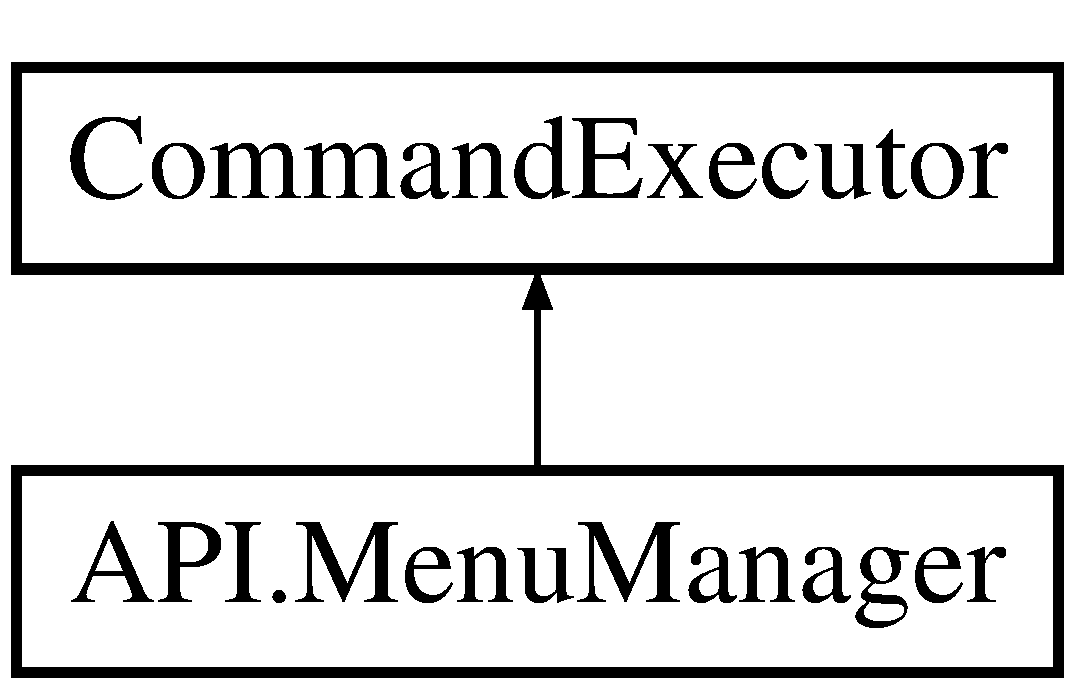
\includegraphics[height=2.000000cm]{class_a_p_i_1_1_menu_manager}
\end{center}
\end{figure}
\subsection*{Public Member Functions}
\begin{DoxyCompactItemize}
\item 
\mbox{\Hypertarget{class_a_p_i_1_1_menu_manager_a340fe9d00b3837983d5d2979e99d8c7f}\label{class_a_p_i_1_1_menu_manager_a340fe9d00b3837983d5d2979e99d8c7f}} 
void {\bfseries save\+Menus} ()
\item 
boolean \hyperlink{class_a_p_i_1_1_menu_manager_a19ba30dd360343792e18b81b621b1a1b}{add\+Menu} (\hyperlink{class_a_p_i_1_1_configurable_menu}{Configurable\+Menu} menu)
\item 
void \hyperlink{class_a_p_i_1_1_menu_manager_a171c35c1ecde734a3f145db60cd02ea4}{delete\+Menu} (\hyperlink{class_a_p_i_1_1_configurable_menu}{Configurable\+Menu} menu)
\item 
void \hyperlink{class_a_p_i_1_1_menu_manager_ae91bcce56f83bdfe318b23521ec19c3d}{delete\+Menu} (String title)
\item 
\mbox{\Hypertarget{class_a_p_i_1_1_menu_manager_a3158467b1e48c0cf367b0dc7abf5e0f8}\label{class_a_p_i_1_1_menu_manager_a3158467b1e48c0cf367b0dc7abf5e0f8}} 
boolean {\bfseries on\+Command} (Command\+Sender sender, Command cmd, String label, String\mbox{[}$\,$\mbox{]} args)
\end{DoxyCompactItemize}
\subsection*{Static Public Member Functions}
\begin{DoxyCompactItemize}
\item 
\mbox{\Hypertarget{class_a_p_i_1_1_menu_manager_a0511013bead3b317121406197845d7b0}\label{class_a_p_i_1_1_menu_manager_a0511013bead3b317121406197845d7b0}} 
static \hyperlink{class_a_p_i_1_1_menu_manager}{Menu\+Manager} {\bfseries get\+Manager} ()
\item 
static \hyperlink{class_a_p_i_1_1_configurable_menu}{Configurable\+Menu} \hyperlink{class_a_p_i_1_1_menu_manager_a42fe754044645b83635c8611ce2f1870}{get\+Menu} (String title)
\item 
static boolean \hyperlink{class_a_p_i_1_1_menu_manager_a79ec953890a2548a05a13b483adb424e}{contains\+Menu} (String title)
\end{DoxyCompactItemize}


\subsection{Member Function Documentation}
\mbox{\Hypertarget{class_a_p_i_1_1_menu_manager_a19ba30dd360343792e18b81b621b1a1b}\label{class_a_p_i_1_1_menu_manager_a19ba30dd360343792e18b81b621b1a1b}} 
\index{A\+P\+I\+::\+Menu\+Manager@{A\+P\+I\+::\+Menu\+Manager}!add\+Menu@{add\+Menu}}
\index{add\+Menu@{add\+Menu}!A\+P\+I\+::\+Menu\+Manager@{A\+P\+I\+::\+Menu\+Manager}}
\subsubsection{\texorpdfstring{add\+Menu()}{addMenu()}}
{\footnotesize\ttfamily boolean A\+P\+I.\+Menu\+Manager.\+add\+Menu (\begin{DoxyParamCaption}\item[{\hyperlink{class_a_p_i_1_1_configurable_menu}{Configurable\+Menu}}]{menu }\end{DoxyParamCaption})\hspace{0.3cm}{\ttfamily [inline]}}

Adds an new menu. 
\begin{DoxyParams}{Parameters}
{\em menu} & the new menu to add. \\
\hline
\end{DoxyParams}
\begin{DoxyReturn}{Returns}
true if added or false if title already exists. 
\end{DoxyReturn}
\mbox{\Hypertarget{class_a_p_i_1_1_menu_manager_a79ec953890a2548a05a13b483adb424e}\label{class_a_p_i_1_1_menu_manager_a79ec953890a2548a05a13b483adb424e}} 
\index{A\+P\+I\+::\+Menu\+Manager@{A\+P\+I\+::\+Menu\+Manager}!contains\+Menu@{contains\+Menu}}
\index{contains\+Menu@{contains\+Menu}!A\+P\+I\+::\+Menu\+Manager@{A\+P\+I\+::\+Menu\+Manager}}
\subsubsection{\texorpdfstring{contains\+Menu()}{containsMenu()}}
{\footnotesize\ttfamily static boolean A\+P\+I.\+Menu\+Manager.\+contains\+Menu (\begin{DoxyParamCaption}\item[{String}]{title }\end{DoxyParamCaption})\hspace{0.3cm}{\ttfamily [inline]}, {\ttfamily [static]}}

Checks if the menu with the same title exists. 
\begin{DoxyParams}{Parameters}
{\em title} & the specified menu title. \\
\hline
\end{DoxyParams}
\begin{DoxyReturn}{Returns}
true if exists or false if doesn\textquotesingle{}t exists. 
\end{DoxyReturn}
\mbox{\Hypertarget{class_a_p_i_1_1_menu_manager_a171c35c1ecde734a3f145db60cd02ea4}\label{class_a_p_i_1_1_menu_manager_a171c35c1ecde734a3f145db60cd02ea4}} 
\index{A\+P\+I\+::\+Menu\+Manager@{A\+P\+I\+::\+Menu\+Manager}!delete\+Menu@{delete\+Menu}}
\index{delete\+Menu@{delete\+Menu}!A\+P\+I\+::\+Menu\+Manager@{A\+P\+I\+::\+Menu\+Manager}}
\subsubsection{\texorpdfstring{delete\+Menu()}{deleteMenu()}\hspace{0.1cm}{\footnotesize\ttfamily [1/2]}}
{\footnotesize\ttfamily void A\+P\+I.\+Menu\+Manager.\+delete\+Menu (\begin{DoxyParamCaption}\item[{\hyperlink{class_a_p_i_1_1_configurable_menu}{Configurable\+Menu}}]{menu }\end{DoxyParamCaption})\hspace{0.3cm}{\ttfamily [inline]}}

Deletes an menu. 
\begin{DoxyParams}{Parameters}
{\em menu} & the menu to delete. \\
\hline
\end{DoxyParams}
\mbox{\Hypertarget{class_a_p_i_1_1_menu_manager_ae91bcce56f83bdfe318b23521ec19c3d}\label{class_a_p_i_1_1_menu_manager_ae91bcce56f83bdfe318b23521ec19c3d}} 
\index{A\+P\+I\+::\+Menu\+Manager@{A\+P\+I\+::\+Menu\+Manager}!delete\+Menu@{delete\+Menu}}
\index{delete\+Menu@{delete\+Menu}!A\+P\+I\+::\+Menu\+Manager@{A\+P\+I\+::\+Menu\+Manager}}
\subsubsection{\texorpdfstring{delete\+Menu()}{deleteMenu()}\hspace{0.1cm}{\footnotesize\ttfamily [2/2]}}
{\footnotesize\ttfamily void A\+P\+I.\+Menu\+Manager.\+delete\+Menu (\begin{DoxyParamCaption}\item[{String}]{title }\end{DoxyParamCaption})\hspace{0.3cm}{\ttfamily [inline]}}

Deletes an menu. 
\begin{DoxyParams}{Parameters}
{\em title} & the menu with the corresponding title. \\
\hline
\end{DoxyParams}
\mbox{\Hypertarget{class_a_p_i_1_1_menu_manager_a42fe754044645b83635c8611ce2f1870}\label{class_a_p_i_1_1_menu_manager_a42fe754044645b83635c8611ce2f1870}} 
\index{A\+P\+I\+::\+Menu\+Manager@{A\+P\+I\+::\+Menu\+Manager}!get\+Menu@{get\+Menu}}
\index{get\+Menu@{get\+Menu}!A\+P\+I\+::\+Menu\+Manager@{A\+P\+I\+::\+Menu\+Manager}}
\subsubsection{\texorpdfstring{get\+Menu()}{getMenu()}}
{\footnotesize\ttfamily static \hyperlink{class_a_p_i_1_1_configurable_menu}{Configurable\+Menu} A\+P\+I.\+Menu\+Manager.\+get\+Menu (\begin{DoxyParamCaption}\item[{String}]{title }\end{DoxyParamCaption})\hspace{0.3cm}{\ttfamily [inline]}, {\ttfamily [static]}}

Gets the menu with the same title as specified. 
\begin{DoxyParams}{Parameters}
{\em title} & the specified menu title. \\
\hline
\end{DoxyParams}
\begin{DoxyReturn}{Returns}
the corresponding menu or null if not found. 
\end{DoxyReturn}


The documentation for this class was generated from the following file\+:\begin{DoxyCompactItemize}
\item 
Configurable\+Menus/src/main/java/\+A\+P\+I/Menu\+Manager.\+java\end{DoxyCompactItemize}

%--- End generated contents ---

% Index
\backmatter
\newpage
\phantomsection
\clearemptydoublepage
\addcontentsline{toc}{chapter}{Index}
\printindex

\end{document}
